\documentclass{beamer}
\usetheme{Berlin}
%Arquivo com os principais pacotes usados e suas descrições.

%%%%%%%%%%%%%%%%%%%%%%%%%%%%%%%%%%%%%%%%%
% 			Idiomas e Acentos			%
%%%%%%%%%%%%%%%%%%%%%%%%%%%%%%%%%%%%%%%%%
\usepackage[brazil]{babel} % Habilita o uso do idioma português do brasil (PT-BR).
\usepackage[T1]{fontenc} 
%\usepackage{fontspec} % Habilita maior variedade de acentos. Pode ser necessario adicionar outros pacotes.
\usepackage{lmodern} % Habilita o uso da font Latin Modern.


%%%%%%%%%%%%%%%%%%%%%%%%%%%%%%%%%%%%%%%%%
% 				TABELAS					%
%%%%%%%%%%%%%%%%%%%%%%%%%%%%%%%%%%%%%%%%%
%\usepackage{tabulary} % Cria tabelas mais facilmente.
%\usepackage{booktabs} % Melhora o visual das tabelas.
%\usepackage[table]{xcolor} % Pacote de cor pra as tabelas.
%\usepackage{caption} % Melhora as legendas de imagens, tabela etc.

%%%%%%%%%%%%%%%%%%%%%%%%%%%%%%%%%%%%%%%%%
% 				IMAGENS					%
%%%%%%%%%%%%%%%%%%%%%%%%%%%%%%%%%%%%%%%%%
%\usepackage{graphicx} % Facilita a inserção de imagens.


%%%%%%%%%%%%%%%%%%%%%%%%%%%%%%%%%%%%%%%%%
% 			CÓDIGO FONTE				%
%%%%%%%%%%%%%%%%%%%%%%%%%%%%%%%%%%%%%%%%%
%Documentação de código fonte.
\usepackage{listings}


%%%%%%%%%%%%%%%%%%%%%%%%%%%%%%%%%%%%%%%%%
% 	Símbolos e Caracteres Matemáticos	%
%%%%%%%%%%%%%%%%%%%%%%%%%%%%%%%%%%%%%%%%%
\usepackage{amsmath}
\usepackage{amssymb}
\usepackage{amsfonts}
%\usepackage{mathspec} %Habilita o uso das fontes e dos caracteres matematicos.


%%%%%%%%%%%%%%%%%%%%%%%%%%%%%%%%%%%%%%%%%
%				ABNT					%
%%%%%%%%%%%%%%%%%%%%%%%%%%%%%%%%%%%%%%%%%
%\usepackage[alf]{abntcite} % Ordena as referencias em ordem alfabética.
\usepackage{url} %Facilita o uso de url. Pode-se usar o comando \url{...}.


%%%%%%%%%%%%%%%%%%%%%%%%%%%%%%%%%%%%%%%%%
% 			Configurações				%
%%%%%%%%%%%%%%%%%%%%%%%%%%%%%%%%%%%%%%%%%
%\captionsetup{justification=centering,labelfont=bf} %Formata a legenda das figuras.
%\graphicspath{{../imgs/}} %Define o diretorio padrão para buscar as imagens da apresentação.  
%\setromanfont[Ligatures=TeX]{Crimson}
%\defaultfontfeatures{Scale=MatchLowercase, Mapping=tex-tex}

%%%%%%%%%%%%%%%%%%%%%%%%%%%%%%%%%%%%%%%%%
%				BEAMER					%
%%%%%%%%%%%%%%%%%%%%%%%%%%%%%%%%%%%%%%%%%
%Define algumas configurações que serão validas para todo o documento.  
\setbeamertemplate{section in toc}[sections numbered]
\setbeamertemplate{subsection in toc}[subsections numbered]
\setbeamertemplate{background canvas}[vertical shading][bottom=blue!3,top=blue!7]
\setbeamertemplate{caption}[numbered]

\usepackage{listings}
\usepackage{color}
\author{Guilherme Augusto de Macedo \and Matheus Liberato Domingues da Silva \and Victor Hugo Carlquist da Silva}

\title{\textsc{Modelo de Banco de Dados para Gerenciamento de Pizzaria: Modelagem e Implementação}}
\date{\today}

\lstset{language=SQL,
	basicstyle = \ttfamily\footnotesize, % Tamanho da fonte do código
	numbers = left, % Posição da numeração das linhas
	numberstyle = \tiny\color{blue}, % Estilo da numeração de linhas
	stepnumber = 1, % Numeração das linhas ocorre a cada quantas linhas?
	numbersep = 10pt, % Distância entre a numeração das linhas e o código
	backgroundcolor = \color{white}, % Cor de fundo
	showspaces = false, % Exibe espaços com um sublinhado
	showstringspaces = false, % Sublinha espaços em Strings
	showtabs = false, % Exibe tabulação com um sublinhado
	frame = l, % Envolve o código com uma moldura, pode ser single ou trBL
	rulecolor = \color{black}, % Cor da moldura
	tabsize = 2, % Configura tabulação em x espaços
	captionpos = b, % Posição do título pode ser t (top) ou b (bottom)
	breaklines = true, % Configura quebra de linha automática
	breakatwhitespace= false, % Configura quebra de linha
	%title = \lstname, % Exibe o nome do arquivo incluido
	%caption = \lstname, % Também é possível usar caption no lugar de title
	keywordstyle = \color{blues}, % Estilo das palavras chaves
	commentstyle = \color{greens}, % Estilo dos Comentários
	stringstyle = \color{reds}, % Estilo de Strings
	escapeinside = {\%*}{*)}, % Permite adicionar comandos LaTeX dentro doseu có digo
	morekeywords ={*,USE,GO} % Se quiser adicionar mais palavras-chave
}

\begin{document}

    \frame{
        \titlepage
    }

	\frame{
        \frametitle{Introdução}
        \begin{itemize}
        	\item Pedidos online;
			\item Clientes podem ou não ter login;
			\item Deliver;
			\item Dependentes;
			\item Admissão e Demissão;
			\item Estoque ;
			\item Log Automático;
			\item Esquema Backup.
    	\end{itemize}
    }
	
	\frame{
        \frametitle{Modelo Conceitual}
		\begin{figure}[h]
			 \centering
			 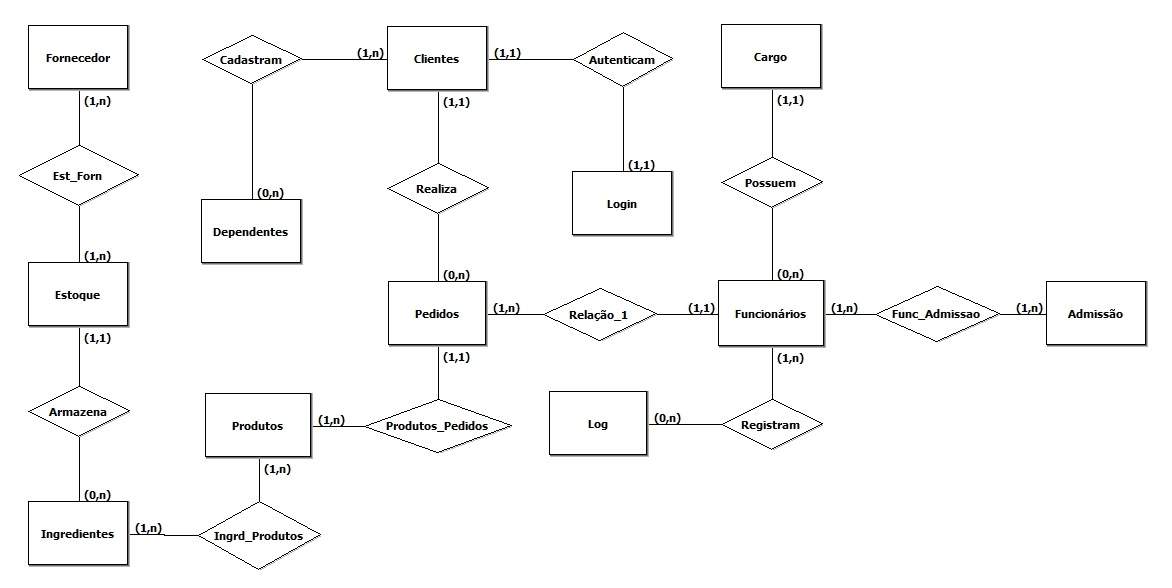
\includegraphics[width=10cm,keepaspectratio]{../BancoDeDadosPizzaria/ModeloConceitual}
			 \caption{Modelo conceitual}
			 \label{ModConceitual}
		\end{figure}
        
    }
	
	\frame{
        \frametitle{Modelo Lógico}
		\begin{figure}[h]
			 \centering
			 \includegraphics[width=10cm,keepaspectratio]{../BancoDeDadosPizzaria/ModeloLógico}
			 \caption{Modelo lógico}
			 \label{ModLogico}
		\end{figure}
    }
	
	% Acho que devemos mostrar apenas dois ou três selects (os mais interessantes)
	% senão não dá tempo.
	\frame{
        \frametitle{Consultas - Select}
		% A Consulta
		\lstinputlisting{sttufs/###.sql}
    }
	
	\frame{
        \frametitle{Consultas - Select}
		% O Resultado
		\begin{figure}[h]
			 \centering
			 \includegraphics[width=10cm,keepaspectratio]{../BancoDeDadosPizzaria/###}
			 \caption{Select ###}
			 \label{Select01}
		\end{figure}
    }
	
	\frame{
        \frametitle{Consultas - Stored Procedures}
		\lstinputlisting{sttufs/###.sql}
    }
	
	\frame{
        \frametitle{Consultas - Stored Procedures}
		% O Resultado
		\begin{figure}[h]
			 \centering
			 \includegraphics[width=10cm,keepaspectratio]{../BancoDeDadosPizzaria/###}
			 \caption{Select ###}
			 \label{Select01}
		\end{figure}
    }
	
	% Qualquer outra coisa que for feita no banco pode entrar aqui.
	
	\frame{
		\frametitle{Considerações finais}
		Apesar de parecer simples, criar um banco de dados para uma pizzaria se mostrou 
		ser uma tarefa cheia de detalhes a se pensar. Ao ser implementado, tornou-se 
		funcional, sendo possível ser utilizado em um ambiente real.
	}
\end{document}
		
